\documentclass[11pt]{article}
\usepackage[margin=1in]{geometry}
\usepackage{amsmath, amssymb, amsthm}
\usepackage{bm}
\usepackage{graphicx}
\usepackage{cite}
\usepackage{tikz}
\usetikzlibrary{arrows.meta, positioning, fit, backgrounds}

\newtheorem{definition}{Definition}
\newtheorem{theorem}{Theorem}
\newtheorem{remark}{Remark}

\title{\textbf{Master Theory Document: Cotangent-Lifted Self-Similar Wreath Recursion and Hybrid Contraction for Hierarchical Power Grid Control}}
\author{Unified Hybrid Hierarchy Formulation}
\date{}

\begin{document}

\maketitle

% =========================================================================
% SECTION 1: MULTI-LAYER GRID HIERARCHY & THREE-LAYER OPERATIONAL FOCUS
% =========================================================================
\section{Hierarchical Power Grid Architecture and Operational Scope}

While the physical hierarchy of an electric power interconnection extends downward to fundamental electromagnetic field equations (Maxwell's PDEs on copper conductors and magnetic cores) and upward to outer economic, regulatory, and policy regimes, this unified control framework focuses on the \textbf{three core operational control layers} bounded between the physical EMT base and the top-level grid optimizer \cite{Sherman2026, Pappas2000, GirardPappas2009}:

\begin{figure}[ht!]
\centering
\resizebox{\textwidth}{!}{%
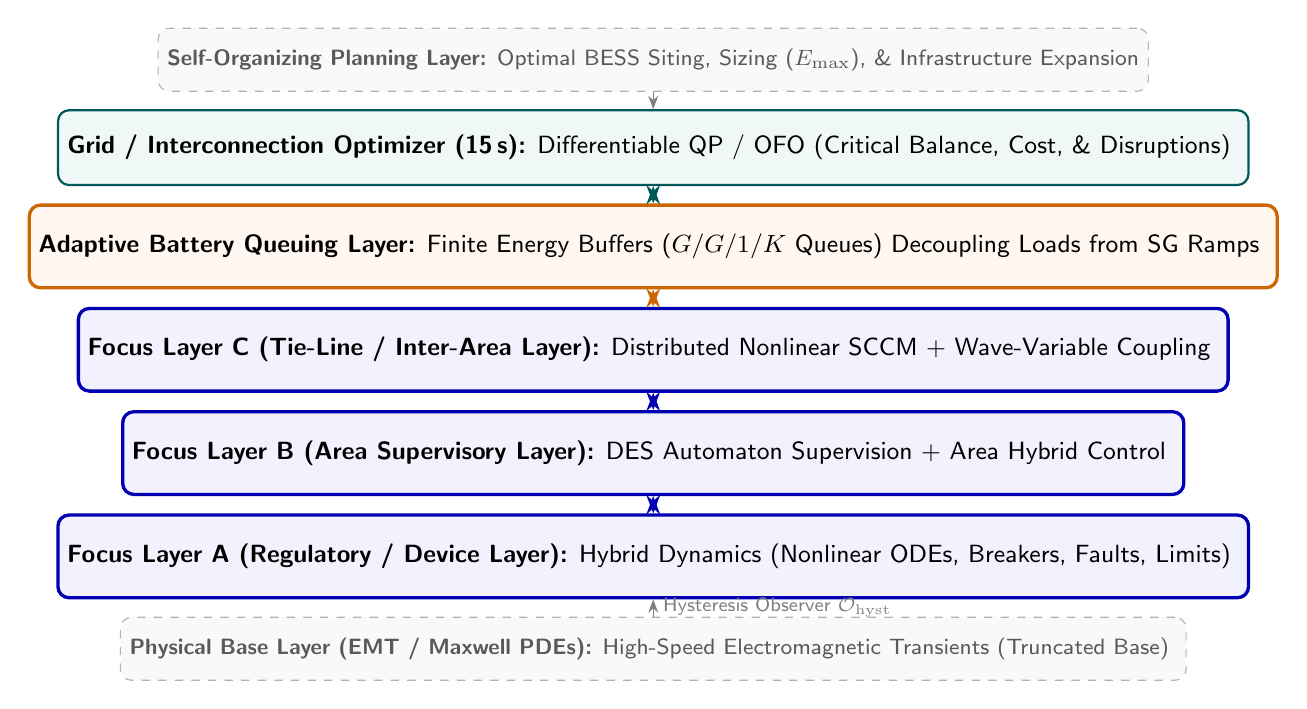
\begin{tikzpicture}[
    >=Stealth,
    layer/.style={
        rectangle, rounded corners=4pt, draw=black!75, thick,
        minimum width=11.0cm, minimum height=0.95cm, align=center, font=\small\sffamily
    },
    focus/.style={
        rectangle, rounded corners=4pt, draw=blue!70!black, very thick, fill=blue!5,
        minimum width=11.0cm, minimum height=1.05cm, align=center, font=\small\sffamily
    },
    queue/.style={
        rectangle, rounded corners=4pt, draw=orange!80!black, very thick, fill=orange!6,
        minimum width=11.0cm, minimum height=1.05cm, align=center, font=\small\sffamily
    },
    outer/.style={
        rectangle, rounded corners=4pt, draw=gray!60, dashed, fill=gray!5,
        minimum width=11.0cm, minimum height=0.80cm, align=center, font=\footnotesize\sffamily, text=gray!70!black
    }
]

\node[outer] (selforg) {\textbf{Self-Organizing Planning Layer:} Optimal BESS Siting, Sizing ($E_{\max}$), \& Infrastructure Expansion};
\node[layer, below=0.22cm of selforg, fill=teal!6, draw=teal!70!black] (grid) {
    \textbf{Grid / Interconnection Optimizer (15\,s):} Differentiable QP / OFO (Critical Balance, Cost, \& Disruptions)
};
\node[queue, below=0.22cm of grid] (adapt) {
    \textbf{Adaptive Battery Queuing Layer:} Finite Energy Buffers ($G/G/1/K$ Queues) Decoupling Loads from SG Ramps
};
\node[focus, below=0.22cm of adapt] (tie) {
    \textbf{Focus Layer C (Tie-Line / Inter-Area Layer):} Distributed Nonlinear SCCM + Wave-Variable Coupling
};
\node[focus, below=0.22cm of tie] (area) {
    \textbf{Focus Layer B (Area Supervisory Layer):} DES Automaton Supervision + Area Hybrid Control
};
\node[focus, below=0.22cm of area] (reg) {
    \textbf{Focus Layer A (Regulatory / Device Layer):} Hybrid Dynamics (Nonlinear ODEs, Breakers, Faults, Limits)
};
\node[outer, below=0.22cm of reg] (emt) {
    \textbf{Physical Base Layer (EMT / Maxwell PDEs):} High-Speed Electromagnetic Transients (Truncated Base)
};

\draw[<->, thick, blue!70!black] (reg.north) -- (area.south);
\draw[<->, thick, blue!70!black] (area.north) -- (tie.south);
\draw[<->, thick, orange!80!black] (tie.north) -- (adapt.south);
\draw[<->, thick, teal!70!black] (adapt.north) -- (grid.south);
\draw[->, dashed, gray] (selforg.south) -- (grid.north);
\draw[->, dashed, gray] (emt.north) -- node[right, font=\scriptsize\sffamily] {Hysteresis Observer $\mathcal{O}_{\mathrm{hyst}}$} (reg.south);

\end{tikzpicture}%
}
\caption{Hierarchical power grid control stack showing the Adaptive Battery Queuing Layer positioned between the 15-second Grid Optimizer and the three fast hybrid control layers, bounded above by the Self-Organizing Planning Layer and below by the truncated EMT base \cite{Sherman2026}.}
\end{figure}

\begin{remark}[Spatial Scale Separation and Truncation]
Each tree depth corresponds to a distinct physical length scale: device/inverter clusters (feet), substation/area buses (miles), inter-area tie-lines (hundreds of miles), and interconnection optimization (regional). Although the algebraic tree $X^*$ is defined recursively without bound, physical modeling truncates at finite depth $n$ (acting on $X^n$) at the EMT/Device interface, where nanosecond electromagnetic wave propagation decouples from millisecond-to-second electromechanical stability.
\end{remark}
\subsection{Adaptive Battery Queuing Layer and Self-Similar Demand Scaling}

Unlike packet-switched communication networks where data packets can be delayed in router memory without altering system physics, electric loads require instantaneous power delivery upon connection. To reconcile instantaneous customer service with slower synchronous generator (SG) ramp limits and 15-second bulk dispatch updates, distributed Battery Energy Storage Systems (BESS) form an \textbf{Adaptive Queuing Layer} directly beneath the grid optimizer.

\paragraph{1. Finite Energy Queues Decoupling Loads from Synchronous Generators:}
From the perspective of bulk synchronous generators, a newly connected load is served immediately by local BESS discharge and remains in an \emph{energy service queue} until bulk SG generation ramps up to relieve the battery and restore its State of Charge ($\mathrm{SoC}$). Modeling each regional BESS cluster as a finite-capacity energy queue ($G/G/1/K$ buffer) with stored energy state $q_i(t) \in [0, E_{\max, i}]$:
\begin{equation}
\dot{q}_i(t) = \eta_{\mathrm{ch}}\, P_{\mathrm{SG}, i}^{\mathrm{del}}(t) - \frac{1}{\eta_{\mathrm{dis}}}\, P_{\mathrm{load}, i}^{\mathrm{net}}(t)
\end{equation}
where $P_{\mathrm{load}, i}^{\mathrm{net}}(t) = P_{\mathrm{load}, i}(t) - P_{\mathrm{DER}, i}(t)$ represents the bursty net demand arrival process and $P_{\mathrm{SG}, i}^{\mathrm{del}}(t)$ represents the scheduled bulk generator service rate. Thus, customers experience zero waiting time, while the BESS buffer absorbs the transient service lag of the bulk SG fleet.

\paragraph{2. Critical Stability Boundary and Absorbing Phase Transition:}
In the sense of Renormalization Group (RG) theory, the interconnected grid operates near a \textbf{critical stability boundary} governed by instantaneous power balance:
\begin{equation}
\Delta P_{\mathrm{margin}}(t) \triangleq \sum_{i=1}^{N} \Big( P_{\mathrm{SG}, i}^{\mathrm{del}}(t) + P_{\mathrm{BESS}, i}^{\max}\big(q_i(t)\big) - P_{\mathrm{load}, i}^{\mathrm{net}}(t) \Big) \ge 0
\end{equation}
As long as $\Delta P_{\mathrm{margin}}(t) \ge 0$ and battery queues avoid depletion ($q_i(t) > 0$), the network remains in the active, contracting operating phase. Conversely, if a burst of demand depletes the local battery queue ($q_i(t) \to 0$) before SG service arrives ($\Delta P_{\mathrm{margin}}(t) < 0$), frequency and voltage collapse drive trajectories across the guard surface into the \textbf{absorbing failure sink $F$} (an absorbing-state phase transition). Above the adaptive layer, the 15-second optimizer manages this critical point alongside generation cost and switching disruption minimization, while the outer \textbf{Self-Organizing Planning Layer} determines optimal BESS siting and queue capacities $E_{\max, i}$ across network buses.

\paragraph{3. Top-Down Self-Similar Traffic vs.\ Bottom-Up Automaton Sequences:}
Aggregate power demand and EV/DER fluctuations exhibit statistical self-similarity and long-range dependence across timescales and spatial aggregation levels (with Hurst parameter $H \in (0.5, 1)$). Positioning the Adaptive Battery Queuing Layer between the 15-second optimizer and the fast hybrid layers connects both directions of the self-similar hierarchy:
\begin{itemize}
    \item \textbf{Top-Down Demand Scaling:} Self-similar demand traffic dictates how variance scales downward across tree depths $v \in X^n$, defining the required Pontryagin inner-erosion headroom ($\mathcal{Y}_i^{\mathrm{phys}} \ominus \mathcal{B}_{\epsilon_i}(0)$) reserved inside each battery queue so burst arrivals do not trigger queue underflow between optimizer ticks.
    \item \textbf{Bottom-Up Symbolic Sequences:} Simultaneously, the lower-layer switching automaton generates self-similar discrete topology sequences via wreath recursion, with the adaptive battery queues acting as a physical RG low-pass filter that absorbs fast switching and load transients locally.
\end{itemize}

% =========================================================================
% SECTION 2: CONTRACTING-CELL BASE TREE & COTANGENT BUNDLE
% =========================================================================
\section{Contraction-Cell Base Tree and Cotangent Fiber Bundle}

To bridge continuous nonlinear dynamics with discrete switching hierarchies, we distinguish between \emph{dynamical contraction} in state space \cite{LohmillerSlotine1998, Shiromoto2018} and \emph{algebraic tree contraction} across hierarchical layers \cite{Nekrashevych2005}.

\begin{definition}[Dynamical Contraction Region and Dual Metric]
Given continuous nonlinear dynamics $\dot{x} = f_w(x, u, \theta)$ in discrete topological mode $w$, a region $\mathcal{C}_w \subset \mathcal{M}$ is a \textbf{contraction region} with rate $\lambda > 0$ if there exists a uniformly positive definite Riemannian metric $M_w(x, \theta) = W_w(x, \theta)^{-1}$ ($\alpha_1 I \preceq M_w \preceq \alpha_2 I$) such that the generalized Jacobian $F_w = \frac{\partial f_w}{\partial x}$ satisfies \cite{LohmillerSlotine1998}:
\begin{equation}
\dot{M}_w(x, \theta) + F_w^\top M_w(x, \theta) + M_w(x, \theta) F_w + 2\lambda M_w(x, \theta) \preceq 0 \qquad \forall x \in \mathcal{C}_w
\end{equation}
The inverse metric $W_w(x, \theta) = M_w(x, \theta)^{-1}$ is introduced purely as a convexification dual variable so that offline synthesis of $W_w$ and $Y_w = K_w W_w$ becomes a convex Linear Matrix Inequality (LMI) \cite{Shiromoto2018}.
\end{definition}

\begin{definition}[Algebraic Contracting Self-Similar Semigroup / Group]
Let $X = \{0, 1, F\}$ denote the per-layer symbolic cell alphabet induced by partitioning $\mathcal{C}_w$ into nominal ($0$), ride-through ($1$), and absorbing fault ($F$) cells. A self-similar semigroup $\mathcal{G} \le \operatorname{End}(X^*)$ (or group $\mathcal{G} \le \operatorname{Aut}(X^*)$ on reversible sub-alphabets) is \textbf{contracting} if there exists a finite subset $\mathcal{N} \subset \mathcal{G}$ (the \emph{nucleus}) such that for every $g \in \mathcal{G}$, there exists a depth $k_0 \ge 0$ satisfying \cite{Nekrashevych2005}:
\begin{equation}
g|_v \in \mathcal{N} \qquad \forall v \in X^* \text{ with } |v| \ge k_0
\end{equation}
\end{definition}

\paragraph{Vertical Fiber Bundle Structure:}
A multi-scale spatial configuration across $n$ truncated layers is represented by a finite word $w = x_1 x_2 \cdots x_n \in X^n$. Over each discrete node $v \in X^n$, attach a $2d$-dimensional fiber $F_v \cong T_{x_v}\mathcal{M} \times T^*_{x_v}\mathcal{M} \cong \mathbb{R}^{2d}$ carrying:
\begin{enumerate}
    \item \textbf{Top-Down Control \& Disaggregation Vectors ($\delta x_v, \delta u_v$):} Propagating setpoints and variational displacements downward across layers.
    \item \textbf{Bottom-Up Margin \& Adjoint Covectors ($\psi_v$):} Propagating reachable-tube sensitivities and safety margins upward to supervisory coordinators (evaluated via backward adjoint integration in an offline or online Digital Twin, as physical grid dissipation prevents direct physical time reversal).
\end{enumerate}

% =========================================================================
% SECTION 3: UNIFIED COTANGENT-LIFTED WREATH RECURSION
% =========================================================================
\section{Unified Cotangent-Lifted Wreath Recursion}

Following Nestruev's algebraic framework \cite{Nestruev2003}, let $\mathcal{O}(\mathcal{M})$ denote the commutative algebra of smooth observables (sensor measurements, tie-line power flows, and bus voltages) on the physical state space. A system transition $g \in \mathcal{G}$ induces an algebra homomorphism $g^* : \mathcal{O}(\mathcal{M}) \to \mathcal{O}(\mathcal{M})$ pulling back observables along trajectories.

\begin{definition}[Cotangent-Lifted Wreath Recursion]
Each elementary switching/evolution generator $g \in \mathcal{G}$ acts simultaneously on the spatial hierarchical address $xw \in X^n$ ($x \in X, w \in X^{n-1}$) and on the attached fiber $\xi_{xw} = (\delta x_{xw}, \psi_{xw})^\top \in F_{xw}$ via the wreath recursion representation \cite{Nekrashevych2005}:
\begin{equation}
\Psi : \mathcal{G} \longrightarrow \big(\mathcal{G} \ltimes \mathrm{GL}(2d, \mathbb{R})\big) \wr_X \operatorname{Trans}(X)
\end{equation}
defined recursively down the hierarchical layers by:
\begin{equation}
g \cdot \big(xw,\, \xi_{xw}\big) = \Big( \pi_g(x)\,(g|_x)(w),\; \Omega_g(x)\, \xi_{xw} \Big)
\end{equation}
where $\pi_g : X \to X$ is the local mode transition, $g|_x \in \mathcal{G}$ is the renormalized section passed to child layer $w$, and $\Omega_g(x)$ transports the forward variational and backward Digital-Twin adjoint fibers across continuous flows $\Phi_g(x)$ and switching saltation operators $\Xi_g(x)$:
\begin{equation}
\Omega_g(x) =
\begin{bmatrix}
\Phi_g(x) & 0 \\
0 & \big(\Xi_g(x)^\top\big)^{-1}
\end{bmatrix}
\end{equation}
\end{definition}

\begin{remark}[Space vs.\ Time Action of Generators]
The tree $X^n$ strictly indexes spatial nesting down the hierarchical layers (not time). A single generator $g$ updates the multi-layer spatial state at a fixed event instant, whereas \textbf{evolution in time} over $[0, T]$ is generated by sequential word composition $g_{t_k} \cdots g_{t_2} g_{t_1}(w_0)$ interspersed with continuous flow intervals.
\end{remark}

\subsection{Nested Sub-Representations: DES, DEVS, and Hybrid Systems}
Under Definition 3, the three classical formalisms sit as nested structural restrictions of $(\mathcal{G}, \Psi)$:
\begin{itemize}
    \item \textbf{Discrete-Event Systems (DES):} Obtained by setting $d = 0$ ($\Omega_g(x) \equiv I_0$), yielding a pure self-similar automaton semigroup acting on $X^n$ \cite{ZhongWonham1990}.
    \item \textbf{Coupled DEVS:} Obtained by equipping $\Psi$ with a scalar temporal scaling cocycle $\gamma_g : X \to \mathbb{R}_+$ governing scale-invariant time-advance updates $ta_{vx} = \gamma_g(x)\,ta_v$ across coupled layers \cite{Zeigler2018}.
    \item \textbf{Hybrid Systems (ODEs + Events):} Realized by the full fiber representation $\Omega_g(x) \in \mathrm{GL}(2d, \mathbb{R})$ with $d = \dim(\mathcal{M})$, coupled with zero-crossing guard surfaces $g_m(x) = 0$ and mode-switching reset maps $x^+ = \Delta_m(x^-)$ at the regulatory layer \cite{Borquez2026}.
\end{itemize}

\paragraph{Contraction Across Discrete Events.}
Discrete switching events are contracted in two distinct mathematical ways depending on whether one analyzes the symbolic event sequence itself or the continuous physical states riding through those events:
\begin{enumerate}
    \item \textbf{Symbolic Contraction (in the Rooted Tree Metric $X^*$):} Even without numerical state values, a discrete automaton contracts symbolically by shrinking the set of distinguishable future trajectories. In the reversible self-similar group setting ($G \le \operatorname{Aut}(X^*)$), this occurs via the \emph{ultrametric tree depth}, where symbolic differences deeper down the word $x_1 x_2 \dots x_n$ carry exponentially smaller weight $2^{-n}$ \cite{Nekrashevych2005}. When passing to an irreversible physical self-similar semigroup ($S \le \operatorname{End}(X^*)$, such as a Renormalization Group coarse-graining step), contraction also occurs via \emph{synchronizing/resetting transitions}---for example, a generator $c$ mapping both \texttt{0} and \texttt{1} into \texttt{0}, collapsing two distinct symbolic paths into a single macroscopic branch.
    \item \textbf{Metric / Cotangent Contraction (Hybrid Dwell-Time):} In a physical power grid, a discrete breaker trip does not occur in isolation; it switches the continuous nonlinear dynamics from $f_{\mathrm{normal}}(x)$ to $f_{\mathrm{fault}}(x)$. At the instant of the switch, the distance between two trajectories jumps by the saltation matrix norm $\mu$ (a numerical stretching factor). Contraction is preserved across the discrete event because the continuous flow between switches contracts at rate $\lambda$ fast enough to dissipate that jump before the next event arrives ($\tau_{\mathrm{dwell}} > \ln(\mu)/\lambda$).
\end{enumerate}
% =========================================================================
% SECTION 4: FINITE-NUCLEUS REACHABILITY & DIGITAL TWIN FAILURE DETECTION
% =========================================================================
\section{Reachable Set Reduction via Contracting Nucleus and Auxiliary Failure Detection}

\paragraph{Topological Partitioning of the Caltech SoCal 28-Bus System:}
In empirical EMT substation studies on the Caltech SoCal 28-Bus distribution dataset \cite{Xie2026SoCal}, the physical network naturally partitions into two hierarchical control areas operating across three voltage levels (16.5\,kV sub-transmission, 2.4\,kV primary distribution, and 480\,V low-voltage secondary):
\begin{itemize}
    \item \textbf{Area 1 (A Side --- Passive Load Feeder):} Supplied by the 16.5\,kV source at Bus 1033 through a $\Delta\text{-Y}$ substation transformer to 2.4\,kV main bus 1034 and primary laterals 1081 and 1117, serving five measured 480\,V secondary load buses (1069, 1106, 1097, 1082, and 1118).
    \item \textbf{Area 2 (B Side --- Inverter-Dominated DER Feeder):} Supplied by the 16.5\,kV source at Bus 1035 through a $\Delta\text{-Y}$ transformer to 2.4\,kV main bus 1036 and primary laterals 1123, 1087, 1168, and 1159, serving five parallel 480\,V load buses (1124, 1088, 1100, 1112, and 1075) alongside inverter-interfaced Distributed Energy Resources (DERs) at 480\,V Bus 1183 (Fuel Cells) and Bus 1175 (Photovoltaics and EV Chargers).
    \item \textbf{Inter-Area Tie-Line Boundary (Six Tie Breakers):} The boundary projection $\Phi_i(x_i)$ spans six tie breakers bridging A Side and B Side: one 2.4\,kV primary tie breaker connecting Bus 1034 to Bus 1036 (\texttt{cb\_143/145}), and five 480\,V secondary tie breakers bridging the parallel load pairs (1118--1124, 1082--1088, 1097--1100, 1106--1112, and 1069--1075).
\end{itemize}

\paragraph{Caltech Substation Nucleus Example:}
Indexed by the 14-breaker topological word $w \in \{0, 1\}^{14}$, operational switching macro-commands across these tie breakers form a finite physical nucleus:
\begin{equation}
\mathcal{N}_{\mathrm{SoCal}} = \big\{ \mathrm{id},\; g_{\mathrm{sub}},\; g_{\mathrm{bus}},\; g_{\mathrm{bank}},\; g_{\mathrm{upgrade}},\; g_{\mathrm{isol}},\; g_{\mathrm{restore}} \big\}
\end{equation}
Involutive operations such as $g_{\mathrm{sub}}$ (\texttt{cb\_146/147} swap) transfer loads across the 480\,V secondary ties, while the structural upgrade $g_{\mathrm{upgrade}}$ (\texttt{cb\_143/145}: $\mathrm{NO} \to \mathrm{NC}$) closes the 2.4\,kV 1034--1036 tie so B-Side DERs at Buses 1183 and 1175 directly support A-Side voltage regulation. Conversely, $g_{\mathrm{isol}}$ (\texttt{cb\_121, 123, swmp\_17-2 NO}; \texttt{cb\_128 NC} at $+8\text{s}$) isolates a 2.4\,kV transformer bank for maintenance downtime while back-feeding 480\,V loads across the secondary tie breakers (increasing series reactance $X_{\mathrm{eq}}$ and widening the projected $(\Delta V, \Delta I)$ reachable tube), followed by the 4-step ordered restoration word $g_{\mathrm{restore}} = g_{\mathrm{swmp\_17-2}} \circ g_{\mathrm{cb\_128}} \circ g_{\mathrm{cb\_123}} \circ g_{\mathrm{cb\_121}}$.

\begin{theorem}[Finite-Nucleus Hybrid Reachable Set Factorization]
Suppose $(\mathcal{G}, \Psi)$ is contracting with finite nucleus $\mathcal{N}$, and continuous flows satisfy $\|\Phi_g(x)\|_{M_w} \le e^{-\lambda \Delta t}$ with hybrid dwell-time factor $\rho_{\mathrm{hybrid}} = \mu_{\max} e^{-\lambda \tau_{\mathrm{dwell}}} < 1$. From any initial multi-layer state $(w_0, \xi_0)$ with $w_0 \in X^n$:
\begin{enumerate}
    \item \textbf{Discrete Event-Time Reachability:} The discrete reachable set $\operatorname{Reach}_{\mathrm{disc}}(w_0)$---encompassing both state-triggered guards and timer-scheduled events (e.g., $+8\text{s}$ bypass closures and $+40\text{s}$ shunt bank switching)---equals the connected orbit of $w_0$ in the finite level-$n$ Schreier graph $\Gamma_n(\mathcal{N}, S)$.
    \item \textbf{Continuous \& Hybrid Tube Bounds:} For every reachable word $w \in \operatorname{Reach}_{\mathrm{disc}}(w_0)$, the continuous physical fiber $\mathcal{R}_{\mathrm{cont}}(w) \subset F_w$ lies inside an invariant geodesic ball of radius $r_\infty = \bar{d}/(1 - \rho_{\mathrm{hybrid}})$ (calibrated empirically via split conformal prediction $q_{1-\alpha}(w)$ \cite{Vovk2005} or verified against Hamilton--Jacobi hybrid safety sets \cite{Borquez2026}), eliminating exponential horizon blowup over $[0, T]$ and as $T \to \infty$.
\end{enumerate}
\end{theorem}

\begin{remark}[Auxiliary Signal Design for Failure Detection During Downtime]
During maintenance downtime (such as Step 07 coordinated isolation), reduced network redundancy masks incipient secondary faults in passive sensor readings. Following Campbell and Nikoukhah \cite{CampbellNikoukhah2004}, small, persistently exciting auxiliary probing signals $u_{\mathrm{aux}}(t)$ are injected through local converter controls (at Buses 1183 and 1175) and processed through an online/offline \textbf{Digital Twin observer} in Nestruev's observable algebra $\mathcal{O}(\mathcal{M})$ \cite{Nestruev2003}. By separating the observable signatures of healthy bypassed topology $f_{\mathrm{isol}}(x)$ from incipient fault modes $f_{\mathrm{fault}}(x)$ within the dwell window $\tau_{\mathrm{dwell}}$, the Digital Twin detects hidden failures without destabilizing the contracting SCCM loop.
\end{remark}

% =========================================================================
% SECTION 5: NON-SMOOTH STRATIFIED MANIFOLDS, DWELL TIME & OBSERVER BRIDGE
% =========================================================================
\section{Hybrid Dwell-Time Contraction on Non-Smooth Manifolds and Observer Bridge}

\paragraph{1. Stratified Non-Smooth Dynamics and Saltation Jump Gain:}
Physical power grids with hard current limits, saturated PLLs, and opening circuit breakers evolve on a \textbf{non-smooth stratified manifold} (piecewise-smooth vector fields $f_w(x)$ separated by codimension-1 switching surfaces $\mathcal{S}_{w \to w'} = \{x : g_{\mathrm{event}}(x) = 0\}$), where classical global smooth manifold theory breaks down \cite{Borquez2026}. To establish contraction across these non-smooth boundaries without requiring global smoothness, we equip each smooth stratum $\mathcal{C}_w$ with its own Riemannian metric $M_w(x, \theta)$ and bridge the discontinuity at $\mathcal{S}_{w \to w'}$ via the \textbf{saltation matrix}:
\begin{equation}
\Xi_{w \to w'}(x) = \frac{\partial \Delta}{\partial x} + \frac{\Big( f_{w'}(\Delta(x)) - \frac{\partial \Delta}{\partial x} f_w(x) \Big) \left( \frac{\partial g_{\mathrm{event}}}{\partial x} \right)^\top}{\left( \frac{\partial g_{\mathrm{event}}}{\partial x} \right)^\top f_w(x) + \frac{\partial g_{\mathrm{event}}}{\partial t}}
\end{equation}
While the state trajectory $x(t)$ remains continuous across the switch ($\Delta(x) = x$), the discontinuous jump in vector field induces a bounded \textbf{saltation jump gain} $\mu_{w \to w'} \triangleq \|\Xi_{w \to w'}(x)\|_{M_w \to M_{w'}} \ge 1$ on variational displacements $\delta x$.

\paragraph{2. Ternary Semigroup Generators and Supervisory Disabling:}
Partition the per-layer alphabet as $X = X_{\mathrm{safe}} \cup \{F\}$, where $X_{\mathrm{safe}} = \{0, 1\}$ and $F$ is an absorbing failure sink representing Critical Clearing Time (CCT) exceedance or PLL loss-of-lock ($|\theta_{\mathrm{PLL}}| \ge \pi/2$). In the illustrative 3-generator nucleus $\mathcal{N} = \{\mathrm{id}, a, b, c\}$:
\begin{itemize}
    \item $a$: Regional tie-line switching toggle ($0 \leftrightarrow 1$, cascading section $b$ to child layers when stressed);
    \item $b$: Severe fault / PLL saturation impulse ($0 \to 1$, $1 \to F$);
    \item $c$: Dissipative emergency damping / battery clamping ($0 \to 0$, $1 \to 0$).
\end{itemize}
Every generator satisfies $\pi_g(F) = F$ and $g|_F = \mathrm{id}$. Under Zhong--Wonham supervisory control \cite{ZhongWonham1990}, state-dependent admissible generator sets $\Sigma_{\mathrm{allowed}}(w)$ \textbf{disable} controllable transitions leading into the unsafe ideal $\mathcal{I}_F = X^* F X^*$ (preventing loss-of-lock while preserving nonblocking reachability). Global hybrid contraction holds whenever consecutive switching events satisfy the minimum dwell-time condition:
\begin{equation}
\tau_{\mathrm{dwell}} > \frac{\ln(\mu_{\max})}{\lambda}, \qquad \rho_{\mathrm{hybrid}} \triangleq \mu_{\max} e^{-\lambda \tau_{\mathrm{dwell}}} < 1
\end{equation}

\paragraph{3. Hysteresis-Regularized Continuous-to-Symbolic EMT Observer:}
To form the upward communication interface between the continuous physical base / EMT waveform $x(t)$ and the Regulatory/Device symbolic state $x_{\mathrm{sym}}(t^+) \in X^n$ without Zeno chattering, the hysteresis observer $\mathcal{O}_{\mathrm{hyst}} : \mathcal{M} \times X^n \to X^n$ enforces deadbands $[\underline{\gamma}_m, \overline{\gamma}_m]$ on each monitored physical observable $I_m(x(t)) \in \mathcal{O}(\mathcal{M})$ \cite{Nestruev2003}:
\begin{equation}
x_{\mathrm{sym}, m}(t^+) =
\begin{cases}
F, & \text{if } I_m(x(t)) \ge \gamma_{\mathrm{crit}, m} \\
1, & \text{if } x_{\mathrm{sym}, m}(t^-) = 0 \text{ and } I_m(x(t)) > \overline{\gamma}_m \\
0, & \text{if } x_{\mathrm{sym}, m}(t^-) = 1 \text{ and } I_m(x(t)) < \underline{\gamma}_m \\
x_{\mathrm{sym}, m}(t^-), & \text{otherwise}
\end{cases}
\end{equation}
guaranteeing a strictly positive physical separation between opposite threshold crossings and projecting the resulting mode-indexed contraction tubes via Pontryagin inner erosion ($\mathcal{Y}_i^{\mathrm{phys}} \ominus \mathcal{B}_{\epsilon_i}(0)$) \cite{Pappas2000, GirardPappas2009} into linear safe bounds $\mathbf{A}_i^{\mathrm{safe}} y_i^{\mathrm{tie}, t} \le \mathbf{b}_i^{\mathrm{safe}}(t)$ for the top-level 15-second optimizer \cite{Sherman2026}.

\subsection{Saltation-Aware Moving Horizon Estimation (MHE) Arrival-Cost Update}

Consider a sliding-window Moving Horizon Estimator operating over a discrete horizon of $N$ samples $[k-N, k]$ to estimate the continuous grid state $x_j \in \mathbb{R}^{n}$ and physical parameters $\theta \in \Theta$:
\begin{equation}
\min_{\{x_j\}_{j=k-N}^{k},\; \hat{\theta} \in \Theta} \;\; \underbrace{\big\| x_{k-N} - \bar{x}_{k-N} \big\|_{P_{k-N}^{-1}}^{2} + \big\| \hat{\theta} - \bar{\theta}_{k-N} \big\|_{Q_{\theta}^{-1}}^{2}}_{\text{Arrival Cost (Prior History)}} + \sum_{j=k-N}^{k-1} \| w_j \|_{Q^{-1}}^{2} + \sum_{j=k-N}^{k} \| v_j \|_{R^{-1}}^{2}
\end{equation}
where $w_j$ and $v_j$ denote process and measurement residuals, respectively, and $(\bar{x}_{k-N}, P_{k-N})$ summarizes historical trajectory information prior to $t_{k-N}$.

\paragraph{1. Hybrid Horizon Partitioning Across Switching Events:}
Suppose a discrete breaker event $w \to w'$ occurs at timestamp $t_e \in (t_{k-N}, t_k)$ straddling sample interval $[t_m, t_{m+1}]$ ($k-N \le m < k$) across a switching surface $\mathcal{S}_{w \to w'} = \{x : g_{\mathrm{event}}(x) = 0\}$. To prevent post-switching estimation lag without discarding prior parameter information, the MHE equality constraints are partitioned at $t_e$:
\begin{equation}
x_{j+1} =
\begin{cases}
\phi_w(t_{j+1}, t_j;\, x_j, u_j, \hat{\theta}) + w_j, & j < m \\
\phi_{w'}\!\Big(t_{m+1}, t_e^{+};\, \Delta\big(\phi_w(t_e^{-}, t_m;\, x_m, u_m, \hat{\theta})\big), u_m, \hat{\theta}\Big) + w_m, & j = m \\
\phi_{w'}(t_{j+1}, t_j;\, x_j, u_j, \hat{\theta}) + w_j, & j > m
\end{cases}
\end{equation}
where $\phi_w$ and $\phi_{w'}$ denote the continuous nonlinear flow maps in the pre- and post-switch topologies, respectively, and $\Delta(\cdot)$ denotes the discrete state reset map.

\paragraph{2. Saltation-Propagated Arrival-Cost Covariance:}
When the switching instant $t_e$ exits the left boundary of the sliding horizon ($t_e \in [t_{k-N}, t_{k-N+1}]$), the arrival-cost prior mean $\bar{x}_{k-N+1}$ and covariance $P_{k-N+1}$ are propagated across the non-smooth discontinuity using the \textbf{hybrid sensitivity transition matrix} $\Psi_{\mathrm{hybrid}}$:
\begin{equation}
\Psi_{\mathrm{hybrid}} \triangleq \Phi_{w'}(t_{k-N+1}, t_e^{+}) \cdot \Xi_{w \to w'}\big(\hat{x}(t_e^{-})\big) \cdot \Phi_w(t_e^{-}, t_{k-N})
\end{equation}
where $\Phi_w, \Phi_{w'}$ are the pre- and post-switch variational flow Jacobians and $\Xi_{w \to w'}(\hat{x}(t_e^{-}))$ is the saltation matrix evaluated at the estimated pre-switch state:
\begin{equation}
\Xi_{w \to w'}(x) = \frac{\partial \Delta}{\partial x} + \frac{\Big( f_{w'}(\Delta(x)) - \frac{\partial \Delta}{\partial x} f_w(x) \Big) \left( \frac{\partial g_{\mathrm{event}}}{\partial x} \right)^{\top}}{\left( \frac{\partial g_{\mathrm{event}}}{\partial x} \right)^{\top} f_w(x) + \frac{\partial g_{\mathrm{event}}}{\partial t}}
\end{equation}
Updating the prior state and covariance via Extended Kalman / Gauss--Newton arrival-cost propagation yields:
\begin{align}
\bar{x}_{k-N+1} &= \phi_{w'}\!\Big(t_{k-N+1}, t_e^{+};\, \Delta\big(\phi_w(t_e^{-}, t_{k-N};\, \hat{x}_{k-N}, \hat{\theta})\big), u_{k-N}, \hat{\theta}\Big) \\
P_{k-N+1} &= \Psi_{\mathrm{hybrid}}\, P_{k-N}\, \Psi_{\mathrm{hybrid}}^{\top} + Q_{\mathrm{hybrid}}
\end{align}
where $Q_{\mathrm{hybrid}}$ incorporates both discrete process noise $Q_d$ and a rank-one covariance inflation term accounting for SCADA switching-timestamp jitter $\sigma_{t_e}^{2}$:
\begin{equation}
Q_{\mathrm{hybrid}} = Q_d + \sigma_{t_e}^{2} \Big( f_{w'}\big(\hat{x}(t_e^{+})\big) - f_w\big(\hat{x}(t_e^{-})\big) \Big)\Big( f_{w'}\big(\hat{x}(t_e^{+})\big) - f_w\big(\hat{x}(t_e^{-})\big) \Big)^{\top}
\end{equation}
\subsection{Two-Saltation-Matrix Hybrid Observer Analysis Under Unknown Jump Times}

When the continuous-to-symbolic observer $\mathcal{O}_{\mathrm{hyst}}$ detects switching events online via continuous output observables $y(t) = h(x(t)) \in \mathcal{O}(\mathcal{M})$ (such as $\Delta V/\Delta t$ or $\Delta I/\Delta t$ threshold crossings) rather than synchronized SCADA timestamps, a non-zero detection latency $\delta t \triangleq t_{\mathrm{detect}} - t_{\mathrm{true}} > 0$ arises between the true physical breaker trip $t_{\mathrm{true}}$ and the observer mode switch $t_{\mathrm{detect}}$.

Following Alleaume, Bernard, and Di Meglio \cite{Alleaume2024}, the estimation error $e(t) = \hat{x}(t) - x(t)$ in a hybrid PEM/MHE or Extended State Kalman Filter (ESKF) observer traverses two sequential non-smooth transitions across each flow-jump cycle:
\begin{equation}
e(t_{\mathrm{detect}}^{+}) = \underbrace{\Xi_2\big(\hat{x}(t_{\mathrm{detect}}^{-})\big)}_{\text{Observer Jump}} \cdot \Phi_{\mathrm{mismatch}}(t_{\mathrm{detect}}, t_{\mathrm{true}}) \cdot \underbrace{\Xi_1\big(x(t_{\mathrm{true}}^{-})\big)}_{\text{Plant Jump}} e(t_{\mathrm{true}}^{-}) + \mathcal{O}(\delta t^2)
\end{equation}
where:
\begin{enumerate}
    \item \textbf{Plant-Jump Saltation Matrix ($\Xi_1$):} Captures the classical variational jump at $t_{\mathrm{true}}$ when the physical grid switches vector fields $f_w \to f_{w'}$ across $g_{\mathrm{plant}}(x) = 0$.
    \item \textbf{Output-Mismatch Saltation Matrix ($\Xi_2$):} Captures the delayed observer mode switch at $t_{\mathrm{detect}}$, accounting for the mismatch between pre- and post-switch output time derivatives $\big(\nabla h \cdot f_{w'}(x) - \nabla h \cdot f_w(x)\big)$ accumulated over $[t_{\mathrm{true}}, t_{\mathrm{detect}}]$.
\end{enumerate}

\paragraph{Observer Stability \& Implementation Equivalence:}
Asymptotic convergence of the hybrid PEM/MHE observer requires joint contractivity of the composite two-matrix cycle operator $\|\Xi_2 \Phi_{\mathrm{mismatch}} \Xi_1\|_{M} \cdot e^{-\lambda_{\mathrm{obs}} \tau_{\mathrm{dwell}}} < 1$, imposing an upper bound $\delta t \le \delta t_{\max}$ on detection latency. In practice, two equivalent mechanisms satisfy this condition:
\begin{itemize}
    \item \textbf{Two-Matrix Covariance Propagation:} Propagate the arrival-cost covariance $P_{k-N+1}$ through both $\Xi_1$ and $\Xi_2$ (replacing heuristic switching-noise inflation $Q_{\mathrm{hybrid}}$ with the exact analytical output-mismatch map).
    \item \textbf{Sliding-Window / Ring-Buffer Rollback:} Utilizing the active MHE horizon $[k-N, k]$ (or a $3$--$5$ sample ESKF ring buffer), roll back to the inflection sample $k - \delta k$ upon detection at $k$, apply the single classical saltation matrix $\Xi_1$ at $t_{\mathrm{true}}$, and re-integrate forward in mode $w'$. This enforces $\delta t = 0$ and reduces $\Xi_2 \equiv I$.
\end{itemize}

\paragraph{3. Anisotropic Uncertainty Preservation and Reachable Tube Coupling:}
Rather than resetting $P_{k-N+1}$ isotropically across a breaker trip (which discards converged parameter estimates $\hat{\theta}$), the congruence transformation $\Xi_{w \to w'} P_{k-N} \Xi_{w \to w'}^{\top}$ stretches uncertainty exclusively along the state subspace excited by the vector-field discontinuity $f_{w'} - f_w$. The spectral radius of $P_{k-N+1}$ immediately bounds the post-switching state estimation error $\Delta x_{\mathrm{MHE}}$, updating the inter-layer mismatch radius $\epsilon_i$ in the Pontryagin inner-eroded constraints $\mathbf{A}_i^{\mathrm{safe}} y_i^{\mathrm{tie}, t} \le \mathbf{b}_i^{\mathrm{safe}}(t)$ without multi-step window lag.
\subsection{Bidirectional Hierarchical Fault Diagnosis via Fiber Pullbacks}

In large multi-area grids, transmitting full microsecond EMT waveforms upward to regional supervisors violates communication bandwidth limits. Instead, fault detection and root-cause isolation operate as a \textbf{bidirectional query--response loop} across the truncated tree $X^n$:

\begin{enumerate}
    \item \textbf{Upward Coarse Event Aggregation (Prefix Projection):} \\
    Let $\Pi_k : X^n \to X^k$ ($1 \le k < n$) denote the truncation projection mapping a fine multi-layer word $w = x_1 \cdots x_k x_{k+1} \cdots x_n$ to its upper-layer prefix $w_{\mathrm{coarse}} = x_1 \cdots x_k$. Upward communication transmits only coarse symbolic transitions $\Pi_k(w) \to \Pi_k(w')$ generated by the hysteresis observer $\mathcal{O}_{\mathrm{hyst}}$.

    \item \textbf{Downward Root-Cause Fiber Query (Preimage Pullback):} \\
    When an upper layer observes an anomalous or stressed prefix $w_{\mathrm{coarse}} \in X^k$ (e.g., Area~1 entering stressed mode \texttt{'1'}), it issues a targeted downward diagnostic query over the \textbf{preimage fiber}:
    \begin{equation}
    \mathcal{F}(w_{\mathrm{coarse}}) \triangleq \Pi_k^{-1}(w_{\mathrm{coarse}}) \cap \operatorname{Reach}_{\mathrm{disc}}(w_0) = \big\{ w \in \operatorname{Reach}_{\mathrm{disc}}(w_0) : \Pi_k(w) = w_{\mathrm{coarse}} \big\}
    \end{equation}
    Ranking candidate leaf configurations $w \in \mathcal{F}(w_{\mathrm{coarse}})$ by their cotangent tube radii $R_k(w)$ and tracing their \textbf{backward Schreier predecessors} $\operatorname{Pred}(w) = \{(w_{\mathrm{prev}}, g) : g(w_{\mathrm{prev}}) = w\}$ isolates the physical root cause:
    \begin{itemize}
        \item \emph{Local Device Fault / Cascade:} Identified when $w$ exhibits stressed or faulted leaf symbols (e.g., \texttt{'11'} or \texttt{'1F'}) reachable via local cascade sections $g|_x$.
        \item \emph{External Tie-Line Stress:} Identified when leaf states remain nominal (e.g., \texttt{'10'} with $x_2 = \texttt{'0'}$) while incoming Schreier edges originate from inter-area power-transfer generators.
    \end{itemize}

    \item \textbf{Active Auxiliary Probing for Ambiguous Fibers:} \\
    Following Sampath et al.\ \cite{Sampath1995} and Campbell and Nikoukhah \cite{CampbellNikoukhah2004}, whenever two distinct fault hypotheses $w_a, w_b \in \mathcal{F}(w_{\mathrm{coarse}})$ produce identical coarse projections and indistinguishable passive observables, the downward query triggers a bounded auxiliary probing signal $u_{\mathrm{aux}}(t)$ at the leaf converter (within the dwell margin $\tau_{\mathrm{dwell}}$) to separate their pullback signatures in $\mathcal{O}(\mathcal{M})$ \cite{Nestruev2003}.
\end{enumerate}

\begin{remark}[Mode-Decoupled Common Contraction Control]
While the hybrid observer $\mathcal{O}_{\mathrm{hyst}}$ and upward Pontryagin bounds $(\mathbf{A}_i^{\mathrm{safe}}, \mathbf{b}_i^{\mathrm{safe}})$ adapt to discrete switching modes $w \in X^n$, the fast inner-loop SCCM feedback law $u_i = u_i^* + K_i(x_i, \hat{\theta}_i)(x_i - x_i^*)$ is intentionally \textbf{mode-decoupled}, synthesized offline via a Common Contraction Metric $M_i(x_i, \hat{\theta}_i)$ valid across all reachable topologies $\mathcal{W}_{\mathrm{safe}}$. Because physical states remain continuous across breaker transitions ($\Delta(x) = x$), decoupling the fast feedback gain from discrete mode switching eliminates gain-chattering transients under observer detection lag $\delta t$, relying on the 15-second optimizer to update feasible equilibria $(x_i^*, u_i^*)$ after topological reconfiguration.
\end{remark}
% =========================================================================
% USER-PROVIDED & RECENT 2026 ARXIV / CONFERENCE REFERENCES
% =========================================================================
\bibliographystyle{IEEEtran}
\bibliography{references}


\end{document}

